\documentclass[12pt, a4paper, twoside, openright]{scrreprt}

\usepackage[utf8]{inputenc}
\usepackage{cite} % optional, for numeric citations

\usepackage{pdfpages}
\usepackage{subfiles}
\usepackage{graphicx}
\usepackage{mathtools}
\usepackage{amsmath}  % For better mathematical typesetting
\usepackage{amsthm}   % For proof environments and theorems
\usepackage{amssymb}  % For additional mathematical symbols
\usepackage{mathrsfs}
% \usepackage{stmaryrd}
\usepackage[colorlinks=true, linkcolor=black, urlcolor=blue, citecolor=blue]{hyperref}
\usepackage{listings}
\usepackage{color}
\usepackage{tikz}
\usetikzlibrary{arrows.meta, positioning}
% \usetikzlibrary{positioning}
\usepackage{enumitem}
\usepackage{graphicx}
\usepackage{bm}
\usepackage{pgfplots}
% \usepackage[
%     backend=biber,     % Wichtig: Legt das Programm zur Verarbeitung fest
%     style=numeric,     % Zitierstil, z.B. numeric, authoryear, alphabetic
%     sorting=nyt        % Sortierreihenfolge der Quellen (Name, Year, Title)
% ]{biblatex}
% \addbibresource{entropy-v19-i07_20250727}

\usepackage[utf8]{inputenc}      % Für Umlaute (ä, ö, ü)
\usepackage[T1]{fontenc}         % Für korrekte Silbentrennung
\usepackage[ngerman, english]{babel}      % Für deutsche Spracheinstellungen

% % Seitenränder anpassen (optional)
\usepackage[left=4cm, right=2.5cm, top=3cm, bottom=3.5cm]{geometry}

\usepackage{scrlayer-scrpage}
\clearpairofpagestyles
\ofoot*{\pagemark}

% GLOBAL FORMATTING CHANGES
\setlength{\parindent}{0pt}        % No paragraph indentation
\setlength{\parskip}{1em}          % Space between paragraphs

% Define theorem style
\theoremstyle{plain}
\newtheorem{theorem}{Theorem}[section]
\newtheorem{proposition}{Proposition}[section]
\newtheorem{lemma}{Lemma}[section]
\newtheorem{corollary}{Corollary}[section]
\theoremstyle{definition}
\newtheorem{definition}{Definition}[section]
\newtheorem{example}{Example}[section]
\newtheorem{remark}{Remark}[section]
\newtheorem{hypothesis}{Hypothesis}[section]


% Extra spacing before and after theorem environments
\makeatletter
\def\thm@space@setup{%
  \thm@preskip=12pt plus 2pt minus 2pt
  \thm@postskip=12pt plus 2pt minus 2pt
}
\makeatother

\definecolor{dkgreen}{rgb}{0,0.6,0}
\definecolor{gray}{rgb}{0.5,0.5,0.5}
\definecolor{mauve}{rgb}{0.58,0,0.82}

\lstset{frame=tb,
  language=Java,
  aboveskip=3mm,
  belowskip=3mm,
  showstringspaces=false,
  columns=flexible,
  basicstyle={\small\ttfamily},
  numbers=none,
  numberstyle=\tiny\color{gray},
  keywordstyle=\color{blue},
  commentstyle=\color{dkgreen},
  stringstyle=\color{mauve},
  breaklines=true,
  breakatwhitespace=true,
  tabsize=3
}



\widowpenalties 1 10000

\title{Criticality in Formal Languages }
\author{Jonas Peters}

\begin{document}
\pagestyle{empty}
\documentclass[../../main.tex]{subfiles}

\begin{document}
\chapter{Model Framework}
    Empirical analysis of \emph{natural language} reveals an interesting relation between the distance of characters in a text and their mutual information.

    \begin{figure}[h]
        \includegraphics*[width=\textwidth]{./natl_pl.png}
        \caption{Decay of mutual information with separation. Source: \cite{e19070299}}
    \end{figure}

    The data show that mutual information tends to decay with distance, but it does so slowly. To be precise, \emph{mutual information in natural language seems to follow a power-law}.

    Thus, models of natural language should show a similar behavior. In order to filter potential models for natural language by their ability for \emph{power-law behavior}, we need a precise definition.

\section{The Framework}
    The tokens, represented by random variables $X_t$, are elements of a finite alphabet $\Sigma$. For every $t$ and every separation $\tau > 0$, we want to bound
    \[
        I(X_t; X_{t + \tau}) \in \Omega(\tau^{-\alpha}), \ I(X_t; X_{t + \tau}) \in \mathcal{O}(\tau^{-\beta}) \quad ,
    \]
    for some fixed $\alpha, \beta \in \mathbb{R}_{>0}$. 
    
    The first condition ensures that the mutual information does not decay too quickly, while the latter ensures that $I(X_t; X_{t + \tau}) \xrightarrow{\tau \to \infty} 0$, just like the data show. We also may replace the latter condition by this implication.

    The importance of the second condition is further emphasized when considering models like the following time-homogenous Markov chain consisting of the two states $A$ and $B$: The probability to transition from $A$ to $A$ is one, and hence the transition probability from $A$ to $B$ is zero. Similarly, starting at state $B$, we can only remain at state $B$.
    
    The pairwise mutual information of this simple model equals a constant. Thus, we can lower bound it by a power-law. However, the problem is that the mutual information does not \emph{decay with distance}. Thus, we conclude that high mutual information alone is not a good indicator for model quality.

\subsection{Model Definition}
    In sequence modeling, a model is typically built from a finite set of rules or parameters defined over an alphabet $\Sigma$. These rules allow us to assign a probability to any finite string. For instance, a time-homogeneous Markov chain uses a fixed transition matrix to define a probability measure over the set of all strings of a given length $n$ (i.e., over $\Sigma^n$) for any $n \in \mathbb{N}$.

    This central idea of a family of finite domains leads to our general definition:

    \begin{definition}[Model over $\Sigma^*$]
        \label{definition:model_over_sigma_star}
        Let $\Sigma$ be a finite alphabet. A model $S$ over $\Sigma^*$ is a function $S: \Sigma^* \mapsto [0, 1]$ that assigns a probability to each finite string $w \in \Sigma^*$, subject to the constraint that for any length $n \in \mathbb{N}$, the probabilities of all strings of that length sum to one:
        \[
            \sum_{w \in \Sigma^n} S(w) = 1 \quad .
        \]
        Furthermore, we denote the restriction of $S$ to strings of length $n$ as $S_n \coloneqq S|_{\Sigma^n}$. The function $S_n: \Sigma^n \to [0,1]$ is thus a probability measure over $\Sigma^n$.
    \end{definition}

    Another strength of this definition is that we don't constrain models by their parameterization. How the models are defined, and how they compute the probabilities is up to them.

    Additionally, we might want to restrain $S$ in order to have reasonable time and space complexity, and to ensure the model is \emph{consistent}, which means that the language of $S_n$ should look \emph{similar} to $S_{n + d}$, whatever this might mean. We also write $w_i$ for $X_i$. We can think of $w$ as a 1-indexed String of random variables.

    We present one strict definition for this \emph{similarity} in the following definition:

    \begin{definition}
        We say $S$ has the \emph{bulk marginal property} iff for every $n \in \mathbb{N}, \ w \in \Sigma^{n}$ it holds true that
        \[
            \sum_{c \in \Sigma} S_{n + 1}(wc) = S_n(w) \quad .
        \]
    \end{definition}

    \begin{lemma}
        \label{lemma:random_variables_do_not_change_with_future_models}
        For every $d \in \mathbb{N}$, let $I \coloneqq [n + d] \setminus [n] = \{ n+1, \dots, n + d \}$. Then, if $S$ has the bulk marginal property, we have for every $w \in \Sigma^{n}$:
        \[
            \sum_{s \in \Sigma^d} S_{n + d}(ws) = S_n(w) \quad .
        \]
    \end{lemma}
    % \vspace{-2.5em}
    \begin{proof}
        We use induction over $d$. The base case directly follows from the definition of the bulk marginal property. Thus, assume the claim holds for some $d \coloneqq k$. Then we have
        \begin{align*}
            \sum_{s \in \Sigma^{k+1}} S_{n + k + 1}(ws) 
            &= \sum_{v \in \Sigma^k} \sum_{c \in \Sigma} S_{n + k + 1}(wvc) \\
            % &= \sum_{v \in \Sigma^k} \left( \sum_{c \in \Sigma} S_{n + k + 1}((wv)c) \right) \\
            &\underset{\text{bulk marginal property}}{=} \sum_{v \in \Sigma^k} S_{n+k}(wv) \\
            &\underset{\text{inductive hypothesis}}{=} S_n(w) \quad ,
        \end{align*}
        which concludes the induction.
    \end{proof}

    \begin{definition}[Induced Bulk Marginal Model]
        \label{def:induced_bulk_marginal_model}
        Based on the model $S$, we can construct an \emph{induced bulk marginal} model $S^*$ by defining $S_n^*$ recursively as 
        \begin{itemize}
            \item $S_1^* \coloneqq S_1$ ,
            \item $S_{n + 1}^*(wc) \coloneqq S_n^*(w) \dfrac{S_{n+1}(wc)}{\sum_{c' \in \Sigma} S_{n+1}(wc')}$ ,
        \end{itemize}
        where $w \in \Sigma^n, c \in \Sigma$.
    \end{definition}

    \begin{remark}
        If $\sum_{c' \in \Sigma} S_{n+1}(wc') = 0$, we might set $S_{n + 1}^*(wc) \coloneqq S_n^*(w) \dfrac{1}{|\Sigma|}$.
    \end{remark}

    \begin{lemma}
        The induced bulk marginal model $S^*$ indeed has the bulk marginal property.
    \end{lemma}
    \vspace{-2.5em}
    \begin{proof}
        We have:
        \begin{align*}
            \sum_{c \in \Sigma} S_{n + 1}^*(wc) 
            &\underset{\text{def of } S^*}{=} \sum_{c \in \Sigma} S_n^*(w) \frac{S_{n+1}(wc)}{\sum_{c' \in \Sigma} S_{n+1}(wc')} \\
            &= S_n^*(w) \cdot \frac{1}{\sum_{c' \in \Sigma} S_{n+1}(wc')} \sum_{c \in \Sigma} S_{n+1}(wc) \\
            &= S_n^*(w) \cdot \frac{\sum_{c \in \Sigma} S_{n+1}(wc)}{\sum_{c' \in \Sigma} S_{n+1}(wc')} \\
            &\overset{\checkmark}{=} S_n^*(w) \quad .
        \end{align*}
    \end{proof}

\subsection{Restricting the Model}
    In order to analyze a group of models for power-law behavior, we first define a model class by imposing specific constraints on our general model definition. To this end, we restrict our general model $S$ by specifying that for each length $n$, the probability distribution $S_n$ is computed by a parameterized \textbf{inference function}, $f_{n, \bm{\theta}_n}: \Sigma^n \to [0, 1]$. Each function is identified by a parameter vector $\bm{\theta}_n$ from a corresponding \textbf{parameter space} $\Theta_n$.

    For the framework to be valid, each function must define a proper probability distribution. We denote this distribution by $S_{n, \bm{\theta}_n}$ and require that:
    \[
        S_{n, \bm{\theta}_n}(w) \coloneqq f_{n, \bm{\theta}_n}(w) \quad \text{and} \quad \sum_{w \in \Sigma^n} f_{n, \bm{\theta}_n}(w) = 1 \quad .
    \]
    This approach defines a \textbf{model class} $\mathcal{S}_n$, which is the set of all distributions that can be generated by the family of inference functions with parameters in $\Theta_n$:
    \[
        \mathcal{S}_n \coloneqq \{ S_{n, \bm{\theta}_n} \mid \bm{\theta}_n \in \Theta_n \} \quad .
    \]
    A complete model $S \equiv (S_n)_{n \in \mathbb{N}}$ is thus specified by an inference function and a corresponding sequence of chosen parameters $(\bm{\theta}_n)_{n \in \mathbb{N}}$.

    \begin{remark}
        The distinction between the inference function $f$ and the distribution $S$ is crucial. Two different functions, $f_{n, \bm{\theta}}$ and $f_{n, \bm{\theta}'}$, might have vastly different time and space complexities even if they compute the exact same distribution (i.e., $S_{n, \bm{\theta}} = S_{n, \bm{\theta}'}$). The complexity is therefore a property of the specific algorithmic implementation and parameterization of $f_{n, \bm{\theta}_n}$.
    \end{remark}


\subsection{Power-Law Behavior}
    Now, we formalize what it means for a model to exhibit power-law behavior. Specifically, we require power-law decay in mutual information with respect to $\tau$ between \emph{any} two variables $X_t$ and $X_{t + \tau}$. This condition must hold for all $t$ and for samples from \emph{any} distribution $S_n$ where $t + \tau \leq n$.

    \begin{definition}
        We define $i_{S_n}(\tau)$ and $I_{S_n}(\tau)$ to be the minimal and maximal mutual information between any two variables of $S_n$ with distance $\tau$. Formally, let $X_t, X_{t + \tau}$ ($t + \tau \leq n$) be random variables sampled from $S_n$. Then:
        % \vspace{-1em}
        \begin{itemize}
            \item $i_{S_n}(\tau) \coloneqq \min_{t \in [n - \tau]} I(X_t; X_{t + \tau}) \quad ,$
            \item $I_{S_n}(\tau) \coloneqq \max_{t \in [n - \tau]} I(X_t; X_{t + \tau}) \quad .$
        \end{itemize}
    \end{definition}

    \begin{definition}[Strong Power-Law Behavior]
        \label{definition:strong_model_power_law_behavior}
        A model $S$ has \emph{strong lower bound power-law behavior} iff there exist constants $c_\alpha, \alpha \in \mathbb{R}_{>0}$ s.t. for every $n \in \mathbb{N}$ it holds true that $i_{S_n}(\tau) \geq c_\alpha \tau^{-\alpha}$. Similarly, $S$ has \emph{upper bound power-law behavior} iff there exist constants $c_\beta, \beta \in \mathbb{R}_{>0}$ s.t. for every $n \in \mathbb{N}$ it holds true that $I_{S_n}(\tau) \leq c_\beta \tau^{-\beta}$. Furthermore, $S$ has \emph{decaying behavior} iff for every $n \in \mathbb{N}$ we have $I_{S_{n + \tau}}(\tau) \xrightarrow{\tau \to \infty} 0$. Lastly, $S$ has \emph{strong power-law behavior} iff it has strong lower bound and upper bound power-law behavior (alternatively decaying behavior instead of upper bound power-law behavior).
    \end{definition}

    \begin{remark}
        For a model $S^*$ with the bulk marginal property we can replace "for every $n \in \mathbb{N}$" in definition~\ref{definition:strong_model_power_law_behavior} with "for $n \to \infty$" thanks to lemma~\ref{lemma:random_variables_do_not_change_with_future_models}.
    \end{remark}

    \begin{proposition}
        Upper bound power-law behavior implies decaying behavior.
    \end{proposition}
    \vspace{-2.5em}
    \begin{proof}
        Assume model $S$ has upper bound power-law behavior. Then there exist constants $c_\beta, \beta \in \mathbb{R}_{>0}$ s.t. for every $n \in \mathbb{N}$ it holds true that $I_{S_n}(\tau) \leq c_\beta \tau^{-\beta}$, especially for $n \coloneqq n' + \tau$. Thus, for every $n' \in \mathbb{N}$:
        \[
            I_{S_{n' + \tau}}(\tau) \leq c_\beta \tau^{-\beta} \xrightarrow{\tau \to \infty} 0 \quad .
        \]
    \end{proof}

    \begin{definition}
        We define $\overline{i_{S_n}}$ to be the minimal mutual information between any two variables over $S_n$ with arbitrary distance $\tau$. Formally, let $X_i, X_j$ ($1 \leq i < j \leq n$) be random variables with distributions defined by $S_n$. Then:
        \[
            \overline{i_{S_n}} \coloneqq \min_{(i, j) \in [n]^2, i < j} I(X_i; X_j) = \min_{\tau \in [n - 1]} i_{S_n}(\tau) \quad .
        \]
    \end{definition}

    \begin{definition}[Weak Power-Law Behavior]
        \label{definition:weak_power_law_behavior}
        A model $S$ has \emph{weak lower bound power-law behavior} iff $\overline{i_{S_n}} \in \Omega(n^{-\alpha})$ for some $\alpha \in \mathbb{R}_{>0}$. Additionally, $S$ has \emph{weak power-law behavior} iff it has weak lower bound and upper bound power-law behavior (alternatively decaying behavior instead of upper bound power-law behavior).
    \end{definition}

    \begin{theorem}[Power-Law Decay for All Tokens in Models with the Bulk Marginal Property]
        \label{theorem:power_law_decay_in_well-behaved_models_with_weak_power-law_behavior}
        Let $S$ be a model that satisfies the bulk marginal property and exhibits weak lower bound power-law behavior. Then, there exists an $\alpha \in \mathbb{R}_{>0}$ s.t. for every $X_t$, $I(X_{t}; X_{t + \tau}) \in \Omega(\tau^{-\alpha})$ (where $X_t$ and $X_{t + \tau}$ are sampled over $S_{t + \tau}$, or, equivalently, any $S_{t + \tau + k}$).
    \end{theorem}
    \vspace{-2.5em}
    \begin{proof}
        Since $S$ has weak lower bound power-law behavior, there exist $\alpha', c' \in \mathbb{R}_{>0}$ s.t. $\overline{i_{S_n}} \geq c' n^{-\alpha'}$. Then, for every $t \in \mathbb{N}$, we have for $n \coloneqq t + \tau$ by the definition of $\overline{i_{S_n}}$:
        \begin{align*}
            I(X_{t}; X_{t + \tau}) &\geq \overline{i_{S_{t + \tau}}} \\
            &\geq c' (t + \tau)^{-\alpha'} \\
            &= c' \tau^{-\alpha'} (\frac{t}{\tau} + 1)^{-\alpha'} \\
            &\geq c' \tau^{-\alpha'} (t + 1)^{-\alpha'} \quad .
        \end{align*}
        Since $S$ is has the bulk marginal property, this inequality holds when sampling over any $S_{t + \tau + k}, \ k \in \mathbb{N}$. Now, set $\alpha \coloneqq \alpha'$ and $c \coloneqq c' (t + 1)^{-\alpha'}$. Note that $\alpha$ does not depend on $t$. Finally, we see that $I(X_{t}; X_{t + \tau}) \geq c \tau^{-\alpha}$. Thus, we get $I(X_{t}; X_{t + \tau}) \in \Omega(\tau^{-\alpha})$.
    \end{proof}

    In other words, mutual information decays polynomially with distance for all tokens, and the constant $\alpha$ is always the same. This sounds like strong power-law behavior, but the issue is that the scalar $c$ depends on $t$ and we cannot lower bound it by constant greater than zero. Hence, the \emph{starting threshold} $I(X_t; X_{t+1})$ can decay to zero for $t \to \infty$.

    \begin{remark}
        If additionally $S$ had decaying behavior, then of course we would also have $I(X_{t}; X_{t + \tau}) \xrightarrow{\tau \to \infty} 0$.
    \end{remark}

    \begin{remark}
        The importance of this implication might depend on the context. However, this theorem proves to be very useful when considering its contraposition. In fact, we will use this contraposition later to disprove weak power-law behavior of hidden Markov models (and hence also strong power-law behavior).
    \end{remark}

    \begin{remark}
        It is crucial for $S$ to have the bulk marginal property in theorem~\ref{theorem:power_law_decay_in_well-behaved_models_with_weak_power-law_behavior}, or else $I(X_{t}; X_{t + \tau})$ might depend on $S_n$, and we cannot exclude \\ $I(X_{t}; X_{t + \tau}) \xrightarrow{n \to \infty} 0$.
    \end{remark}

\pagebreak
    \begin{proposition}
        \label{proposition:strong_slbplb_implies_wlbplb}
        Strong lower bound power-law behavior implies weak lower bound power-law behavior.
    \end{proposition}
    \vspace{-2.5em}
    \begin{proof}
        Assume model $S$ has strong lower bound power-law behavior. Thus, it follows that there exist $c_\alpha, \alpha \in \mathbb{R}_{>0}$ s.t. for all $n \in \mathbb{N}$ we have that $i_{S_n}(\tau) \geq c_\alpha \tau^{-\alpha}$. Hence:
        \begin{align*}
            \overline{i_{S_n}} &= \min_{\tau \in [n - 1]} i_{S_n}(\tau) \\
            &\geq \min_{\tau \in [n - 1]} c_\alpha \tau^{-\alpha} \\
            &\geq c_\alpha (n - 1)^{-\alpha} \\
            &= c_\alpha n^{-\alpha} (1 - \frac{1}{n})^{-\alpha} \\
            &\geq c_\alpha n^{-\alpha} 1^{-\alpha} \\
            &= c_\alpha n^{-\alpha} \quad .
        \end{align*}
        It follows that $\overline{i_{S_n}} \in \Omega(n^{-\alpha})$, and hence $S$ has weak lower bound power-law behavior.
    \end{proof}

    \begin{remark}
        Weak lower bound power-law behavior does \emph{not} imply strong lower bound power-law behavior, not even for models with the bulk marginal property. To see this, note that we might have  $i_{S_n}(1) \xrightarrow{n \to \infty} 0$ for some models with weak lower bound power-law behavior. ($S_n$ may force $i_{S_n}(1)$ to decay to $0$ for $n \to \infty$ because of weak correlations of consecutive tokens very late in the sequence.) The proof of theorem~\ref{theorem:power_law_decay_in_well-behaved_models_with_weak_power-law_behavior} fails when defining $c$, as it depends on $t$.
    \end{remark}

    \begin{remark}
        If $S$ has decaying behavior, we cannot prove that $S$ has strong lower bound power-law behavior by bounding $\overline{i_{S_{t + \tau}}}$ (using $\overline{i_{S_{t + \tau}}} \leq i_{S_{t + \tau}}(\tau)$), as we have for every $\tau \in \mathbb{N}$:
        \[
            0 \leq \overline{i_{S_{t + \tau}}} \leq I_{S_{t + \tau}}(t) \xrightarrow{t \to \infty} 0 \quad .
        \]
    \end{remark}

    % \begin{definition}
    %     \label{definition:large_scale_time_invariance}
    %     A model $S$ is called \emph{large scale time invariant} iff there exists a vector $\bm{\mu} \in [0,1]^\Sigma$ s.t. for all $a \in \Sigma$ we have
    %     \[
    %         P(X_t = a) \xrightarrow{t \to \infty} \bm{\mu}_a \quad ,
    %     \]
    %     where $X_t$ is sampled over any $S_{t + k}, k \in \mathbb{N}$.
    % \end{definition}
\end{document}
\cleardoublepage

\newpage
\subfile{chapters/abstract/sub.tex}
\cleardoublepage

\newpage
\pagestyle{scrheadings}
\tableofcontents
\cleardoublepage

\subfile{chapters/model_framework/sub.tex}
\subfile{chapters/power_law_model/sub.tex}
\subfile{chapters/regular_grammar/sub.tex}

\appendix
\subfile{chapters/technical_details/sub.tex}

% \cleardoublepage
\phantomsection
\addcontentsline{toc}{chapter}{Bibliography}
\bibliographystyle{plain}  % or 'abbrv', 'unsrt', 'ieeetr', etc.
\bibliography{entropy-v19-i07_20250727}
% \clearpage
% \printbibliography[heading=bibintoc]

\subfile{chapters/ki/sub.tex}

\pagestyle{empty}
\cleardoublepage

\includepdf[pages=-, pagecommand={}]{erklaerung.pdf}

\cleardoublepage
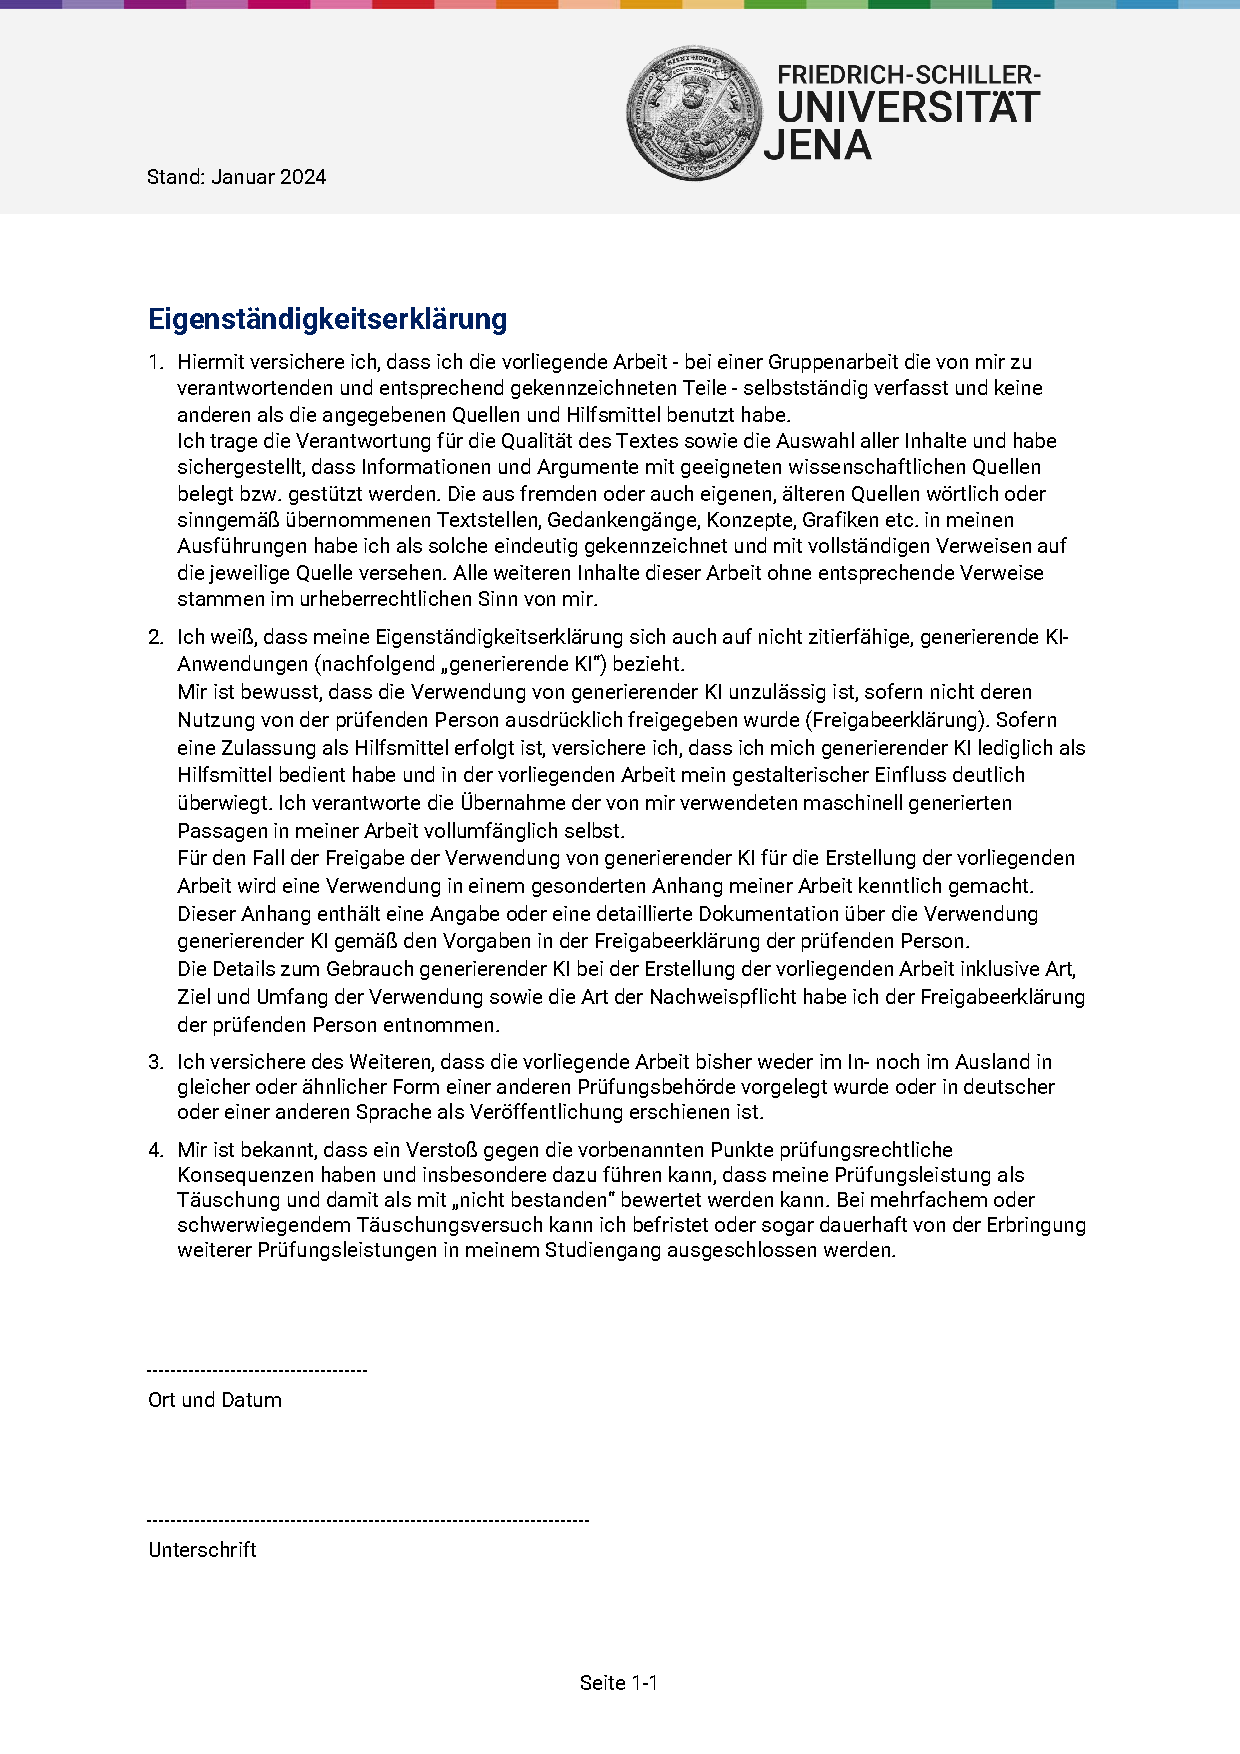
\includepdf[pages=-, pagecommand={}]{freigabe.pdf}
\end{document}